\documentclass[a4paper, 11pt]{article}

\usepackage[english]{babel}
\usepackage{float}
\usepackage[utf8]{inputenc}
\usepackage[left=2cm, top=3cm, text={17cm, 24cm}]{geometry}
\usepackage{times}
\usepackage{amsmath}
\usepackage{graphicx}
\usepackage[hyphens]{url}
\usepackage[unicode, colorlinks, hypertexnames=false, citecolor=red]{hyperref}
% \usepackage[english, boxed]{algorithm2e}
\usepackage[perpage]{footmisc}
\usepackage[inkscapeformat=pdf]{svg}
\usepackage{hyperref}% http://ctan.org/pkg/hyperref
\usepackage{tikz}

\title{blank}
\author{xstahl01 }
\date{December 2024}

\begin{document}
%%%%%%%%%%%%%%%%%%%%%%%%%%%%%%%% Titulní stránka %%%%%%%%%%%%%%%%%%%%%%%%%%%
\begin{titlepage}
    \begin{center}
        
\includegraphics[width=0.77 \linewidth]{include/FIT_logo.pdf}

        \vspace{\stretch{0.382}}

        \Huge{Mikroprocesorové a vestavěné systémy} \\
        \LARGE{\textbf{Řízení servo/krokového motoru pomocí H-můstku}} \\
        \Large{}

        \vspace{\stretch{0.618}}
    \end{center}

    \begin{minipage}{0.5 \textwidth}
        \Large
        \today
    \end{minipage}
    \hfill
    \begin{minipage}[r]{0.5 \textwidth}
        \Large
        \begin{tabular}{ll}
            \textbf{Peter Stáhl} & \textbf{(xstahl01)}
        \end{tabular}
    \end{minipage}
\end{titlepage}


%%%%%%%%%%%%%%%%%%%%%%%%%%%%%%%% Obsah %%%%%%%%%%%%%%%%%%%%%%%%%%%%%%%%%%%%%
\clearpage
\pagenumbering{roman}
\setcounter{page}{1}
\tableofcontents


%%%%%%%%%%%%%%%%%%%%%%%%%%%%%%%% Úvod %%%%%%%%%%%%%%%%%%%%%%%%%%%%%%%%%%%%%%
\clearpage
\pagenumbering{arabic}
\setcounter{page}{1}

\section{Úvod}
Táto dokumentácia sa zaoberá využitím servo a krokového motora za použitia mikrokontroléru ESP32 Wemos D1 R32. Tieto motory sú známe svojou presnosťou a širokým spektrom aplikácií v priemysle, od automatizácie po robotiku. 

Cieľom tejto dokumentácie je priblížiť svet servo a krokových motorov, ich presné fungovanie čitateľovi a zlepšiť teda porozumenie týchto súčiastok, ktoré sa bežne objavujú v našom svete.

Motory sa vo svojej podstate vyznačujú jednoduchým princíom – vykonávať otáčavý pohyb. V praxi je však dôležité pochopiť, ako tento pohyb vzniká a aké technológie umožňujú jeho precíznu kontrolu. V nasledujúcej dokumentácii preto postupne rozoberiem teoretické základy, navrhnem riešenie a popíšem jeho samotnú implementáciu.
%%%%%%%%%%%%%%%%%%%%%%%%%%%%%%%% Rozbor a návrh riešenia %%%%%%%%%%%%%%%%%%%%%%%%%%%%%%%%%%%%%%

\clearpage
\section{Rozbor a návrh riešenia}
Úlohou tejto kapoly je detailnejšie vysvetlenie jednotlivých motorov, ich fungovanie a spôsob ako ich dokážeme ovládať pomocou mikrokontroléru ESP32.  

\subsection{Krokový motor}
Krokové motory sú efektívne zariadenia, ktoré často vieme nájsť v elektrotechnickom a strojáresnkom priemysle. Ich schopnosť vyknávať presné pohyby z nich robí ideálny nástroj pre aplikácie vyžadujúce vysokú presnosť a kontrolu. Ako už názov napovedá, vykonávajú pohyb v krokoch. Tento typ motora je navrhnutý tak, aby sa otáčal o presne definované uhly (kroky) pri každom signále, čo umožňuje veľmi presné ovládanie polohy. 
Princíp fungovania krokového motora spočíva v premene elektrickej energie na magnetickú energiu, ktorá otáča samotnú hriadeľ motora. Hriadeľ motora musí byť teda vyrobená z materiálu, ktorý reaguje na magnetické javy. Samotné otáčanie je vykonávané prúdením elektrickej energie v cievkach motora, ktoré vytvárajú magnetické pole okolo samotnej cievky. Toto pole pri prúdení elektrického prúdu priťahuje hriadeľ a vytvára točivý magnetický pohyb. Pohyb hriadele teda zabezpečujú cievky uložené v kruhovom rozpoložení a ich opakovaný stav vypínania a zapínania. Pri ovládaní krokových motorov pomocou mikrokontrolera, je potrebné následne využiť ovládacie logické obvody, ktoré zabezpečia presnú synchronizáciu jednotlivých cievok. Túto funkcionalitu zaisťuje komponenta H-mostík. 

\subsection{H-mostík}
H-mostík je elektronický obvod používaný na riadenie smeru a rýchlosti otáčania jednosmerných motorov. Jeho názov vychádza z typického zapojenia, ktoré pripomína písmeno "H". Tento obvod umožňuje prúdenie elektrickej energie cez krokový motor. Hlavnou funkcionalitou h-mostíku je schopnosť premeny elektrickej polarity prichádzajúcej do zariadenia, čím zaisťuje rotáciu krokového motora do oboch smerov.

\subsection{Servo motor}
Servo motory sú špeciálnym typom elektrických motorov, ktoré sú navrhnuté na presné ovládanie polohy. Na rozdiel od krokových motorov, ktoré vykonávajú pohyb v presne definovaných krokoch, servo motory používajú pulzné šírkové modulácie (PWM) na riadenie svojej pozície. PWM signál určuje, ako dlho má byť signál "vysoký" (HIGH) v rámci jednocyklického impulzu, čo priamo ovplyvňuje cieľovú pozíciu hriadelu. Napríklad PWM signál s šírkou 1,5 ms typicky reprezentuje neutrálnu pozíciu 90°. Týmto spôsobom môžu dosiahnuť veľmi presné a plynulé pohyby v rozsahu, ktorý je obvykle od 0 do 180 stupňov, čo je prípad, ktorým sa zaoberá táto dokumentácia. Tento typ Servo motora je často regulovaní fyzickou prekážkou aby sa servo motor nedostal za hranice jeho funkčnosti, pričom existujú aj Servo motory, ktoré dokážu rotovať 360 stupňov.

\subsection{Návrh riešenia}
Na demonštráciu príkladu jednotlivých motor a ich použitie použijem mikrokontrolér ESP32 Wemos D1. Krokový motor  28BYJ-48, ktorý je ovládaný štvorfázovým režimom. Tento režim zaručuje plynulé otáčanie a vysokú presnosť, keďže motor vykonáva kroky o uhle 5,625° na krok, čo znamená, že vykoná celú otáčku 64 krokmi. H-mostík L9110S ako ovládač krokévho motora a servomotor umožňujúci sa točiť od 0 do 180 stupňov. 
Bude teda nutné vytvoriť prepojenie medzi krokovým motorom a H-mostíkom. Z H-mostíku vytvoriť prepojenie do mikrokontroléru tak aby mikrokontrolér dokázal rotovať samotný krokový motor. Zároveň musí byť súčasne možné ovládať servo motor pomocou PWM signálu. Samotný návrh teda nie je nejak komplikovaný.

%%%%%%%%%%%%%%%%%%%%%%%%%%%%%%%% Vlastné riešenie %%%%%%%%%%%%%%%%%%%%%%%%%%%%%%%%%%%%%%
\clearpage
\section{Vlastné riešenie}
V tejto časti je mojou úlohou popísať každý aspekt vývoj návrhu prezentovaného v predošlej kapitole. Hlavnou úlohou bude popis samotnej implementácia z aspketu programovania mikrokontroléru s využitím teoretických poznatkov, ktoré som popísal v rozbore dokumentácie. 
\subsection{Programovacie prostredie}
Ako programovacie prostredie som využil integrované vývojové prostredie PlatformIO ako rozšírenie textového editoru VS Code. Hlavnou výhodou tohto prostredia je jeho univerzálnosť pracovať s rozličnými mikrokontrolérmi, teda aj s mojím použitým mikrokontrolérom ESP32 Wemos D1 R32. Jednou z veľkých výhod tohto prostredia, ktoré prišla vhod bola automatizovaný import naištalovaných knížníc pre môj projekt. To zaisťovalo, že pri nahrávaní binárneho kódu, do kontroleru prostredie nahralo aj pribalené knižnice a samotné nahrávanie binárného kódu pomocou prostredia. 
\subsection{Uživateľský kontrolér}
Podstatou môjho riešenia bolo oboznámiť užívateľa s krokovým a servo motor. Zároveň bolo potrebné aby samotný užívateľ bol schopný ovladať tieto motory v reálnom čase a nie len ukázať nejaký skript pohybu. Môj zámer bol zahrnúť užívateľa do samotného ovladánia. 
Bolo potrebné vymyslieť nejaký typ kontroleru, ktorý by užívateľ dokázal interagovať. Jednou s možností na, ktoré som nepristúpil bolo využitie fyzických kontrolérov, ako sú potenciometre a spínače. Naopak som sa rozhodol pre viacej komponentovo ľahšie riešenie a využil som čo môj mikrokontroler ponúkal. Jedná sa o zabudovaní WiFi modul, ktorý som nakonfiguroval do módu prístupového bodu (Access Point). Užívateľ je schopný sa vytvoriť bezdrótové pripojenie cez prehliadač a ovládať tak jednotlivé motory. 
Po pripojení na sieť, môže užívateľ vidieť jednoduchú HTML stránku obsahujúcu pár základných komponentov na ovladánie motor ako je potenciometer na ovládanie servomotora, posúvný selektor pre výber rýchlosti a tlačítka ovlyvňujúce konanie krokvého motoru, ako aj veľa ďalších informácií o samotných zariadeniach. Toto riešenie bolo dosiahnuté pomocou knižnice WebServer.h, kde sa nastavili kredenciály, vytvorila sa entita serveru, ktorá sa následne nakonfigurovala. Mikrokontrolér obsluhuje požiadavky od klienkta v niekoľkých základných endpointoch.
Vďaka tomu riešeniu je jednoduché demonštrovať použitie samotných motorov.

\subsection{Krokový motor}
Pre správnu implementáciu krokového motora je potrebné brať do úvahy teoretický základ ohľadom tohto typu motora. Ak chcem vytvoriť otáčavý pohyb motra, musím vyvolať podnet pre zopnutie kroku. Takýto krok je výsledkom zopnutia elektrického vynutia v motore. Pohyb krokového motora teda je sekvenciou presného usporiadania elektrických impulzov, ktoré sú privádzané na jednotlivé cievky motora. Tento princíp umožňuje nielen presnú kontrolu uhla natočenia, ale aj schopnosť zadefinovať konkrétnu polohu hriadeľa.

Základnou myšlienkou pri práci s krokovým motorom je vytvárať sekvenciu elektrických signálov, ktoré sú privádzané na porty H-mostíka v správnom poradí. Táto sekvencia musí byť v súlade s typom motora a jeho pracovným režimom, v mojom prípade teda sa jedná o 4-fázový motor. Každý krok motora zodpovedá jednej konkrétnej kombinácii aktívnych a neaktívnych portov. Pre implementáciu týchto krokov sa využíva cyklus (\texttt{for loop}), ktorý postupne prepína medzi stavmi podľa preddefinovanej sekvencie. Každý z týchto stavov spôsobí krok motora o uhol. V mojom prípade sa jedna celistvá otáčka vykoná v 64 krokoch teda teto uhol pre konkrétny krokový motor je 5.625 stupňa.
Pri ovládaní unipolárneho krokového motora v 4-fázovom režime sa motor postupne prepína medzi štyrmi rôznymi kombináciami stavov na výstupných pinoch. Každá fáza reprezentuje jednu konkrétnu kombináciu napájania vinutí motora. Tento režim zabezpečuje plynulé otáčanie rotora. Tento cyklus sa opakuje, pričom poradie sa môže otočiť, aby sa rotor pohyboval opačným smerom.
\begin{figure}[H]
    \centering
    \[
    \begin{array}{|l|l|l|l|l|}
    \hline
    \textbf{krok} & \textbf{IN1} & \textbf{IN2} & \textbf{IN3} & \textbf{IN4}\\ \hline
    \textbf{1} & \textbf{1} & \textbf{0} & \textbf{1} & \textbf{0}\\ \hline
    \textbf{2} & \textbf{0} & \textbf{1} & \textbf{1} & \textbf{0}\\ \hline
    \textbf{3} & \textbf{0} & \textbf{1} & \textbf{0} & \textbf{1}\\ \hline
    \textbf{4} & \textbf{1} & \textbf{0} & \textbf{0} & \textbf{1}\\ \hline
    \end{array}
    \]
    \caption{Parameter values}
\end{figure}
Pre výpočet krokov sledujem rýchlosť prepínania stavov. To je ovplyvňovanie funkciou sleep, ktorá spomaluje točenie sa krokového motoru. Táto hodnota je teda vypočítanavná na monitorovania počtu za čas(\texttt{stepInterval}) a následného výpočtu počtu krokov za minútu. Hodnota ja následne zobrazovaná v rotáciách za minútu.


\subsection{Servo motor}
Impelemntácia Servo motora je relatívne jednoduchou záležitosťou. Je potrebné dodať elektrickú energiu pre prácu samotnému motoru, ktorá je spostredkovaná cez samotný mikrokontroler, definovať mikrokontroléru, že má očakávať entitu servomotora, na čo poslúžila dodukovaná knižnicu a nakoniec zadefinovať samotný digitálny pin, pomocou, ktoré bude uskutočnená komunikácia do Servo motoru PWM signálom. Keďže ide o značne jednoduché zariadenie, nie je možné monitorovať aktivitu samotného motora a ani určit jeho polohu pri novou zapojení. Zo strany Servo motora neexistuje odozva, ktorou by sme sa vedeli dozvedieť nejakú monitorovaciu štatistiku. Správa servo motora bola teda celá riešená interne v mikrokontroléri. Mikrokotrolér si po vyslaní signálu do motora, ukladá túto hodnotu do flash pamäťa, pomocou knižnice EEPROM.h. Táto knižnica využíva technológiu "non-volatile memory", čo je typ pamäťe, ktorý nie je závislý od energie. Vďaka tejto vlastnosti si dokáže mikrokontrolér pamätať poslednú polohu servomotora pri reštarte systému ako aj po vypnutí. 



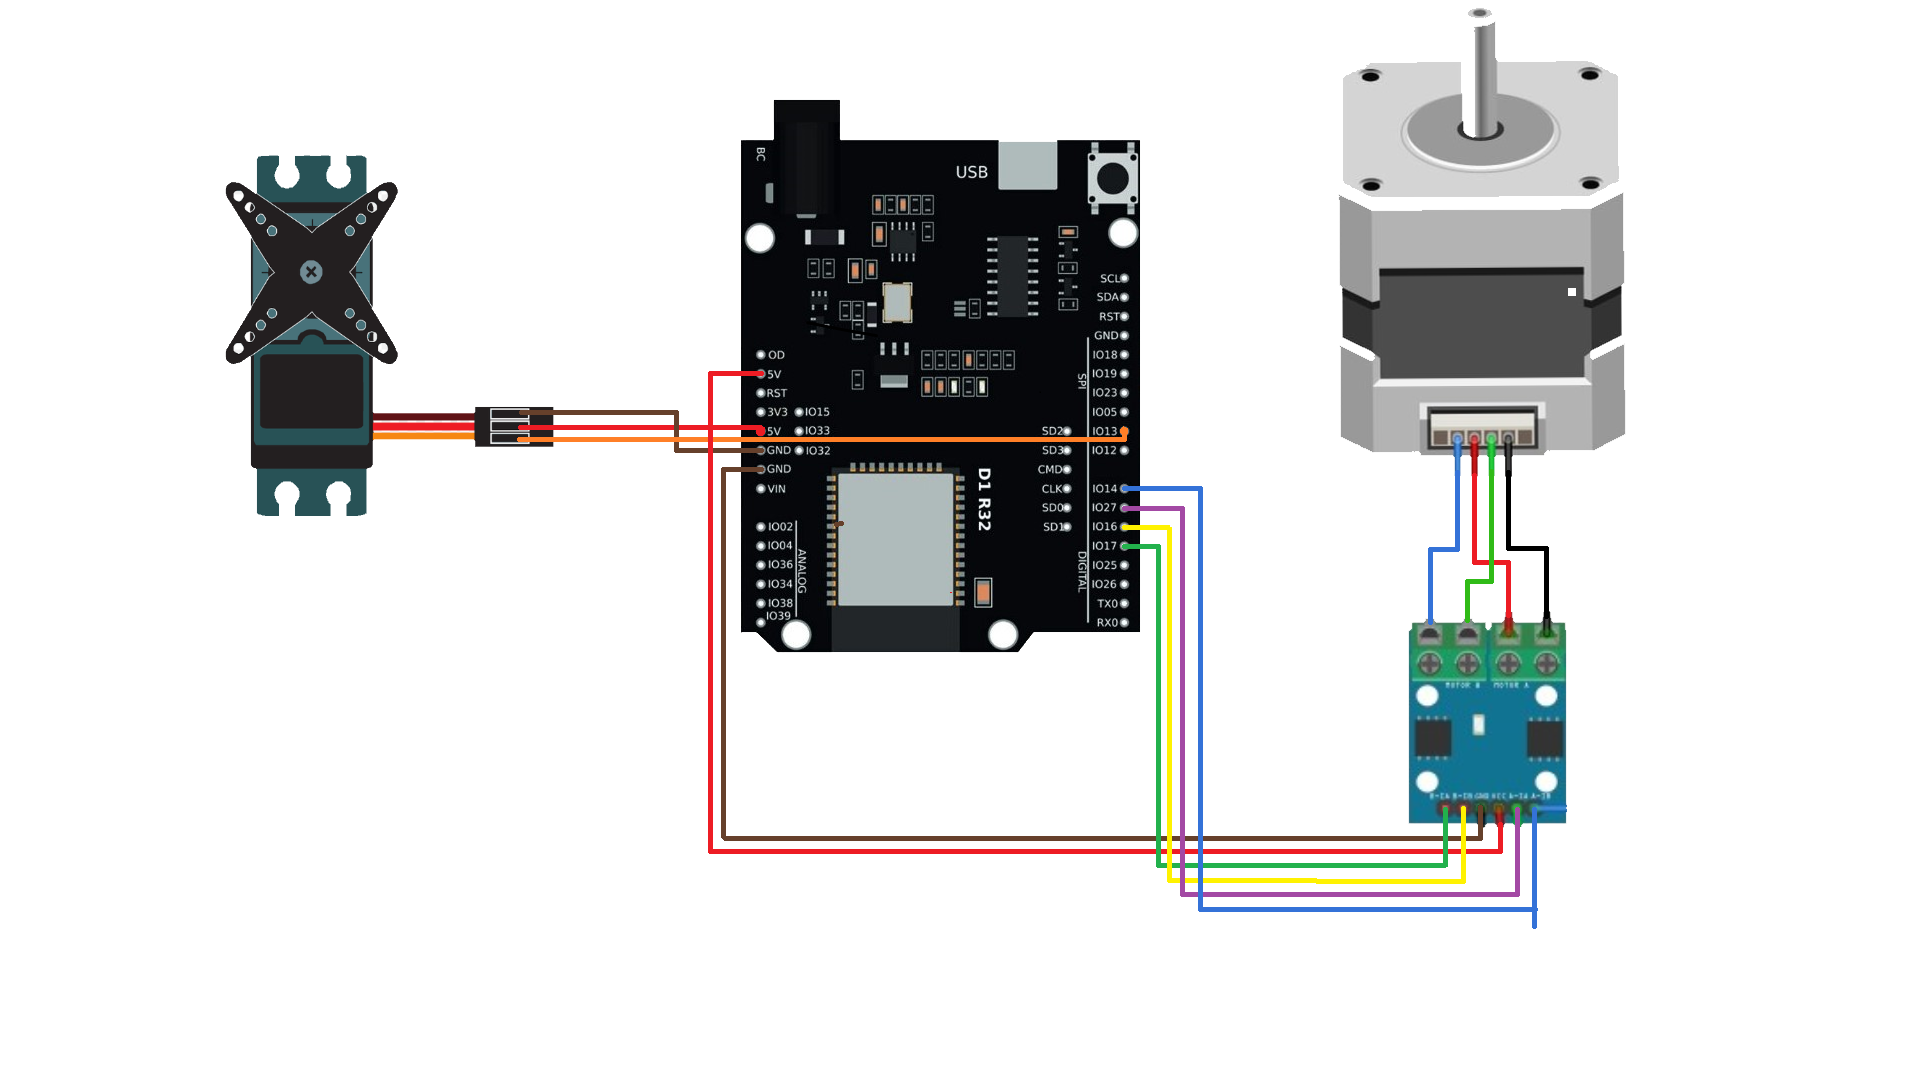
\includegraphics[width=0.9 \linewidth]{include/462556003_559687976836752_7762418375852550792_n.png}
%%%%%%%%%%%%%%%%%%%%%%%%%%%%%%%% Záverečné zhodnotenie %%%%%%%%%%%%%%%%%%%%%%%%%%%%%%%%%%%%%%

\clearpage
\section{Záverečné zhodnotenie}
Po otestovaní celej implementácie som dospel k záveru, že moja práca splnila očakávania, ktoré som si stanovil na začiatku projektu. Cieľom bolo demonštrovať základné použitie servomotoru a krokového motora pomocou mikrokontroléra Wemos D1 R32 s bezdrôtovým ovládaním prostredníctvom technológie WiFi. Považujem túto implementáciu za dostatočnú ako základné riešenie. Zároveň by som rád poukázal na možnosti ďalšieho rozvoja projektu. Implementácia komplexnejších metód, ako je použitie Watchdog Timer-u, zlepšenie prioritizácie úloh pomocou FreeRTOS a celkové monitorovanie systému, by mohli výrazne zvýšiť výkon a stabilitu systému. Tieto vylepšenia by mohli byť obzvlášť užitočné v aplikáciách, kde je potrebná vysoká spoľahlivosť a presnosť. Implementácia spomenutých metód by sa hodila na okrajové pripády, kde by bolo pre mikrokontrolér lepšie stratégia a managment vlastných prostredkov. 

%%%%%%%%%%%%%%%%%%%%%%%%%%%%%%%% Citace %%%%%%%%%%%%%%%%%%%%%%%%%%%%%%%%%%%%
\clearpage
\begin{thebibliography}{9}
\bibitem{dtp}{https://forum.arduino.cc/t/issue-using-wemos-with-servo-library/559377
}
\bibitem{dtp}{\em jkb-git:}
               {\bf ESP32Servo} \\
               https://github.com/jkb-git/ESP32Servo
\bibitem{dtp}{\em randomnerdtutorials.com:}
                {\bf ESP32 Access Point Web Server}\\
                https://randomnerdtutorials.com/esp32-access-point-ap-web-server/
\bibitem{dtp}{\em hadex-návod}:{\bf L9110 2-CHANNEL MOTOR DRIVER} https://www.hadex.cz/navody/m513a.pdf
\bibitem{dtp}{https://forum.arduino.cc/t/solved-controlling-28byj-48-bipolar-mod-with-l9110s/608054
}
\bibitem{dtp}{\em Dejan:}{\bf Stepper Motors and Arduino – The Ultimate Guide} \\
https://howtomechatronics.com/tutorials/arduino/stepper-motors-and-arduino-the-ultimate-guide/
\bibitem{dtp}{\em Sabins Civil Engineering:}{\bf How does a Stepper Motor work?}\\
https://www.youtube.com/watch?v=eyqwLiowZiU
\end{thebibliography}
\bibliographystyle{ieeetr}
\end{document}
